\section{Transition networks {\bf{(Reik)}} } \label{sec:TransitionNt}
The construction of the transition network depends on a proper phase space partition. For instance, we first mesh the phase space with box of equal sizes following the traditional idea of fractal dimension computations \cite{Grassberger1983PRL,Grassberger1983PLA} or complexity measures \cite{Crutchfield1989}. Then each partition is labeled with $\pi_i$ and regarded as a vertex in the network. The connectivity between partition $\pi_i$ and $\pi_j$ is then represented by the transition frequency following the temporal order of observations. Alternatively, one may define a partition as a ``state" based on a symbolic representation of time series, for instance, ordinal patterns of the series \cite{Li2008,McCullough2015}. Transforming the time series into a transition network is a process of mapping the temporal informaiton into a Markov chain to obtain a compressed or simplified representation of the original dynamics. 

	\subsection{Markov chains}
	In the terminology of Markov chain modeling \cite{Nicolis2005}, these partition algorithms generally map time series data to a Markov chain by defining nodes as some set of states that span the time series points, and allocating directed edges based on temporal succession that represent transitional probabilities based on the source data. Therefore, indicators of dynamics are derived from the transition matrix \cite{Nicolis2005}. 
	
	\subsection{Symbolic encoding of time series}
	Coarse-graining the range of values in a time series into a suitable set of classes (``symbols") $\{\pi_1, \dots , \pi_k \}$ allows considering the transition probabilities $w_{\alpha,\beta} = p (x_{i+1} \in \pi_\beta | x_i \in \pi_\alpha)$ between these classes in terms of a weighted and directed network. Therefore, the first step of this approach is to applying a suitable symbolic discretization to the phase space of the studied system. The next step is to explicitly use the temporal order of observations, i.e., their connectivity, to represent causality relationships contained in the dynamics of the observed dynamical system, which hence results in a time directed transition network. The directed network is represented by a weighted matrix $W = \{w_{\alpha, \beta} \}, \alpha, \beta \in [1, \cdots, k]$. Note that for a trajectory that does not leave a finite volume in phase space, there is only a finite number of discrete ``states" $\pi_i$ with a given minimum size in phase space. This implies the presence of absorbing or recurrent states in the resulting transition network. 
	
	The transition probability approach is well suited for identifying such ``states" (i.e. regions in phase space) that have a special importance for the causal evolution of the studied system in terms of betweenness centrality $b_v$ and related measures. Moreover, the resulting networks do not only depend on a single parameter, but on the specific definition of the full set of classes. Note, however, that coarse graining might be a valid approach in case of noisy real-world time series, where extraction of dynamically relevant information hidden by noise can be supported by grouping the data. In contrast to the other approaches for constructing complex networks from time series, the topology of transition networks depends on the specific choice of discretization. In the next sections, we give some examples.
		
		\subsubsection{Threshold-based coarse-graining}
		Note that meshing the phase space with equal size $\varepsilon$ is a threshold-based coarse-graining of the original system. Note that quantile mapping discretizing continuous time series shares much similarity with the threshold based coarse graining technique \cite{Liu2016}. In \cite{Donner2011}, we have illustrated an example in obtaining a transition network from time series of the Lorenz system. The transition behavior among different partitions is characterized by state transition matrix $W$, which is weighted and each entry $W_{ij}$ is estimated by the transition frequency from state $i$ to $j$. Traditionally, the transition entropy is simply the Shannon entropy of the weight matrix $W$, which is used to characterize the changes of the underlying system. 
		
		We note that the temporal information is lost after the coarse graining and the transition frequency matrix $W$ is estimated over the entire time series. Therefore, the resulting ordinal transition network is static representations \cite{Weng2017}. Inspired by the current ideas of temporal networks, Weng {\emph {et al.}} proposed to construct a temporal network from time series by unfolding temporal information $t$ into an additional topological dimension. More specifically, a transition from node $i$ to $j$ is established whenever the trajectory flow performs a transition from $i$ to $j$ at time $t$ which is denoted as ($i \to j; t$). By adding the additional time axis to the transition route, the consecutive memory network is constructed by introducing the memory factor $\tau$ and Weng {\textit{ et al.}} further proposed the memory entropy analysis to characterize the memory effect of the observed time series. The identified memory effect can accurately differentiate various types of time series including white noise, $1/f$ noise, AR model, periodic and chaotic time series. 
		
		\subsubsection{Order pattern-based coarse graining}
		There is a growing number of works in transforming time series into networks by ordinal partitions of time series \cite{Small2013,McCullough2015,Kulp2016b,McCullough2017b,Small2018}.  A series of systematic investigations of ordinal methods has been conducted in irregularly sampled time series \cite{Kulp2016a,McCullough2016,Sakellariou2016}, which shows high potential for studies of experimental observation data from climate sciences \cite{Eroglu2016}. In this method, the first step is to embed a one-dimensional time series $\{x(t)\}$ into phase space by using techniques from traditional time delay embedding, i.e., a proper choice of embedding dimension $D_x$ and time delay $\tau$. Then, embedded points in phase space are mapped to nodes in the network space according to its rank order and links are allocated between nodes based on temporal succession on the trajectory. In Fig. \ref{fig:rosTNm}, we show an example of ordinal partition network using the algorithms of \cite{McCullough2015}. 
\begin{figure}[ht]
	\centering
	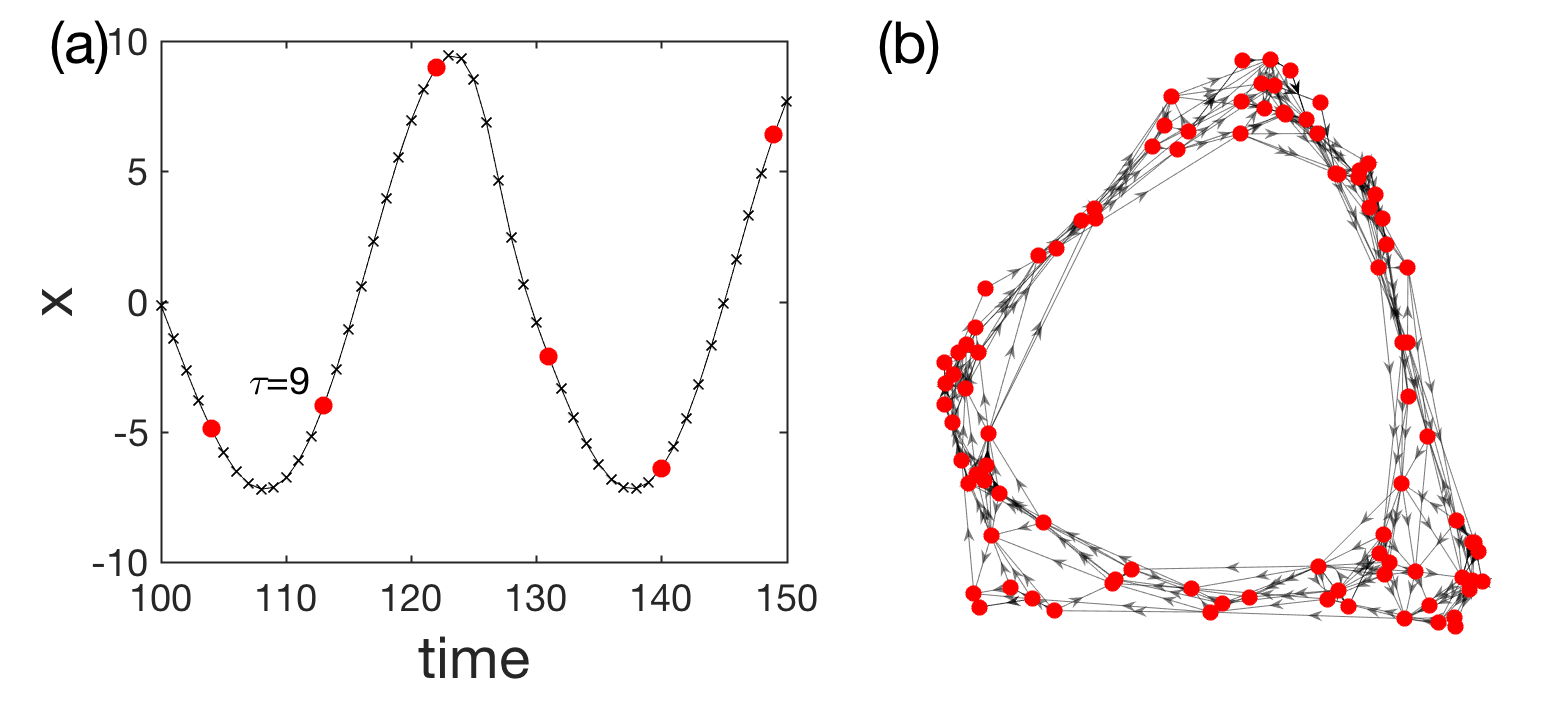
\includegraphics[width=\columnwidth]{Chapter05_TransitionNt/rosslerOPexample.eps}
\caption{(a) illustration of permutation symbols from a time series of the R\"ossler attractor ($a = 0.165$). Assume $\tau = 9$ and $D_x= 6$. The embedded vector is highlighted by red color $\vec{x}_{104} = \{x_{104}, x_{113}, x_{122}, x_{131}, x_{140}, x_{149} \}$ and its corresponding pattern is defined by the rank ordering $\pi_{104} = \{5, 1, 2, 4, 6, 3\}$. (b) ordinal pattern transition network (isolated vertices and self-loops are excluded for the visualization purpose). Directed edges are denoted by arrows. Reproduced from \cite{McCullough2015}. \label{fig:rosTNm}}
\end{figure}
		
		In \cite{McCullough2015}, McCullough {\textit{et al}} illustrated the construction algorithm in detail by the R\"ossler system and find that periodic dynamics translate to ring structures whereas chaotic time series translate to band or tube-like structures -- thereby indicating that this algorithm generates networks whose structure is sensitive to system dynamics. Furthermore, it is demonstrated that simple network measures including the mean out degree and variance of out degrees can track changes in the dynamical behaviour in a manner comparable to the largest Lyapunov exponent \cite{McCullough2015}. Therefore, these results show that measures of transition networks have the potential to be useful as indicators for dynamical discrimination and for detecting change points. 
		
		Note that the embedding dimension $D_x$ and time delay $\tau$ are two important parameters for constructing ordinal partition networks, in particular having crucial impacts on the appearance of forbidden order patterns \cite{Kulp2016b,McCullough2016,Sakellariou2016}. The selection of time delay $\tau$ must be chosen in relation to the sampling rate for continuous systems. The authors proposed using a time delay $\tau > 1$ \cite{Sun2014}. In \cite{McCullough2015}, they proposed to select these two parameters by traditional methods used for time series embedding, for instance, the first zero of the autocorrelation of the time series because it provides a sufficiently good phase space reconstruction for the R\"ossler time series. While there does not yet exist a robust metric for determining the correct choice of $D_x$, in the cases time series of the R\"ossler system they found that networks with the most visually intuitive structure often correspond with peak values of degree variance with respect to $D_x$. In addition, it was demonstrated that the range $6 \leq D_x \leq 10$ was the most useful when using simple network measures to track changes in dynamics \cite{McCullough2015}. Note that the choice of $D_x$ also determines the level of simplification of the original phase space by ordinal partitions. 
		
		Most of the recent works have focused only on univariate time series $\{x(t)\}$. However, the generalization to multivariate time series remains largely untouched. Most of the observable phenomena in the empirical sciences are of a multivariate nature. For instance, assets in stock markets are observed simultaneously and their joint development is analyzed to better understand tendencies. In climate science, multiple observations (temperature, pressure, precipitation, human activities etc, from different locations) are the basis of reliable predictions for the future climate conditions. 
		
		In \cite{Zhang2017b}, they propose to construct ordinal partition transition networks from multivariate (high dimensional) data. Given a scalar time series $\{x(t)\}$ which is produced by a deterministic dynamical system, the order structure of the time series depends on the embedding dimension $D_x$ and time delay $\tau$. Let us start with embedding dimension $D_x = 2$. Neglecting equality, we have two relations between $x(t)$ and $x(t + \tau)$, namely, two symbol sequences representing order patterns $\pi_{x}$:
\begin{equation} \label{piX2D_eq}
\pi_{x} (t) =  \begin{cases}
 1 & \text {if} \; x(t) < x(t + \tau), \\
 0 & \text {if} \; x(t) > x(t + \tau). 
\end{cases}
\end{equation}
In \cite{Small2013}, Small {\textit{et al}} used a fixed lag $\tau = 1$ for embedding and we follow this idea. By this choice, the order pattern $\pi_x^{1}$ captures the increasing trend, respectively, $\pi_x^{0}$ corresponds to the decreasing trend of the time series. This definition is equivalent to considering the signs of the increments $\Delta x(t) = x(t+1) - x(t)$ by a first-order difference of the original series. 

		Generalizing the above idea to the case of three dimensional time series $(x(t), y(t), z(t))$, we first obtain the increment series $(\Delta x(t), \Delta y(t), \Delta z(t))$. Then the order patterns are defined by the combinations of signs of $\Delta x(t), \Delta y(t)$ and $\Delta z(t)$. In particular, the ordinal pattern $\Pi(t) \in (\pi_1, \cdots, \pi_i), i = 1, \cdots, 8$ of a three dimensional time series $(x(t), y(t), z(t))$ is enumerated in Tab. \ref{tab:3D}. 
\begin{table}
\centering
\begin{tabular}{|c|c|c|c|c|c|c|c|c|}
\hline
$\Pi$      & $\pi_1$ & $\pi_2$ & $\pi_3$ & $\pi_4$ & $\pi_5$ & $\pi_6$ & $\pi_7$
& $\pi_8$\\
\hline
$\Delta x$ & $\pi_x^{1}, + $ & $\pi_x^{1}, + $ & $\pi_x^{1}, +$ &
$\pi_x^{1}, +$ & $\pi_x^{0}, - $ & $\pi_x^{0}, - $ &
$\pi_x^{0}, -$ & $\pi_x^{0}, -$\\
\hline
$\Delta y$ & $\pi_y^{1}, + $ & $\pi_y^{1}, + $ & $\pi_y^{0}, -$ &
$\pi_y^{0}, -$ & $\pi_y^{1}, + $ & $\pi_y^{1}, + $ &
$\pi_y^{0}, -$ & $\pi_y^{0}, -$\\
\hline
$\Delta z$ & $\pi_z^{1}, + $ & $\pi_z^{0}, - $ & $\pi_z^{1}, +$ &
$\pi_z^{0}, -$ & $\pi_z^{1}, + $ & $\pi_z^{0}, - $ &
$\pi_z^{1}, +$ & $\pi_z^{0}, -$\\
\hline
\end{tabular}
\caption{Order patterns in three dimensional time series $(x(t), y(t), z(t))$. 
\label{tab:3D}}
\end{table}
Therefore, the dimension of order pattern $\Pi(t)$ for an $n$-dimensional time series $(\{x_1\}(t), \ldots, \{x_n\}(t))$ is $D = 2^{n}$ since each component has either increasing or decreasing trend at time $t$. 

		Noting that we consider the increments between two consecutive time points of each measurement in the space of multi measurements, which captures the dynamic properties of the multi-variate time series in its associated velocity space (difference space). Therefore, time delay $\tau$ in the order pattern definition (Eq. \eqref{piX2D_eq}) has rather a different interpretation with the time delay that is often used in embedding. We can certainly generalize the discussion to the case of time delays larger than 1 (i.e., $\tau > 1$) and embedding dimension $D_x  > 2$ for each variable (measurement), but we think that the physical meaning in terms of dynamics becomes ambiguous for multivariate time series.  

		In addition, the resulting ordinal pattern transition network utilizes nullclines to obtain phase space partitions of the systems. As shown in Fig. \ref{fig:rosslerTwoA}(a), the chaotic R\"ossler system is color coded by the ordinal pattern partitions and the corresponding transition network in shown in Fig. \ref{fig:rosslerTwoA}b. 
\begin{figure}[ht]
	\centering
	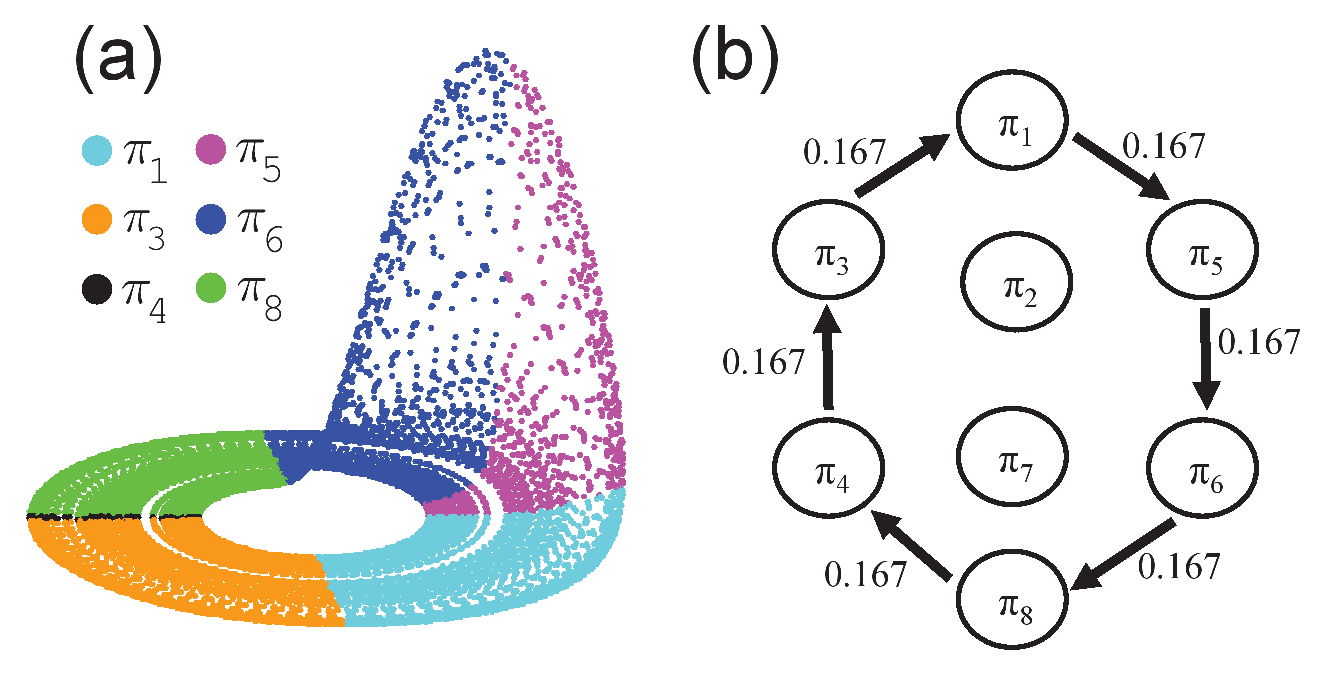
\includegraphics[width=0.7\columnwidth]{Chapter05_TransitionNt/rossler_0165N.eps}

\caption{(a) R\"ossler attractor in phase space color coded by order patterns ($a = 0.165$), (b) ordinal pattern transition network (self-loops are excluded). \label{fig:rosslerTwoA}}
\end{figure}

		In order to emphasize the importance of non-self transitions between ordinal patterns, we remove the self-loops, which is typical of most research work on complex networks \cite{Costa2007}. Furthermore, we remove self-loops before computing the weighted matrix $W$ to keep the normalization $\sum_{i,j}^{2^n} w_{ij} = 1$. Note that self-loops should not be expected with large amounts in stochastic processes. 
		
		Given the observations that different occurrence frequencies of ordinal patterns $p(\pi_i)$ and their transitions $w_{i,j}$, two Shannon entropies are defined as 
		\begin{align} \label{eq:Ho}
		\mathcal{H}_O &= - \sum_{i=1}^{2^n} p(\pi_i) \log_2 p(\pi_i) , \\ \label{eq:Ht}
		\mathcal{H}_T &= - \sum_{i,j=1}^{2^{n}} w_{ij} \log_2 w_{ij}. 
		\end{align}
		In the terminologies of \cite{McCullough2017b}, $\mathcal{H}_{O}$ characterizes the vertext (node) complexity and $\mathcal{H}_{T}$ is for the edge (link) transitional complexity, both of which have been shown useful for characterizing synchronization transition dynamics \cite{Zhang2017b}. Note that Eq. \eqref{eq:Ht} measures the transitional complexity of the ordinal patterns, but in a slightly different way of normalizations as used in \cite{McCullough2017b,Small2018}. 

		\subsubsection{Cross and joint ordinal transition networks} 
		The method of \cite{Zhang2017b} has been further generalized to construct cross and joint ordinal partition transition networks for two coupled systems \cite{Guo2018}. Let us start with an example of a single chaotic R\"ossler system as represented by three variables $(x_1(t), y_1(t), z_1(t))$. The ordinal pattern transition network is reconstructed based on the signs of the increments of each each variables $(\Delta x_1(t), \Delta y_1(t), \Delta z_1(t))$, where $\Delta x_1(t) = x_1(t+1) - x_1(t)$, $\Delta y_1(t) = y_1(t+1) - y_1(t)$, and $\Delta z_1(t) = z_1(t+1) - z_1(t)$. The definition of patterns $\Pi(t) \in (\pi_1, \cdots, \pi_i), i = 1, \cdots, 8$ are enumerated in Tab. \ref{tab:3D}. For two coupled systems, we have further time series from the other system as represented by $(x_2(t), y_2(t), z_2(t))$. 
		
		A cross ordinal pattern transition network (COPT) compares the relative speeds between two systems by the signs of $(\Delta x_1(t) - \Delta x_2(t)), (\Delta y_1(t) - \Delta y_2(t))$ and $(\Delta z_1(t) - \Delta z_2(t))$. The pattern definitions of a COPT are shown in Tab. \ref{tab:3DCOPT}. An example of COPT is reconstructed for two coupled R\"ossler system in a non-sync regime \cite{Guo2018}, which is shown in Fig. \ref{fig:rosCOPT}(a). 
\begin{table}[htb]
\centering
\begin{tabular}{|c|c|c|c|c|c|c|c|c|}
\hline
$\Pi$      & $\pi_1$ & $\pi_2$ & $\pi_3$ & $\pi_4$ & $\pi_5$ & $\pi_6$ & $\pi_7$
& $\pi_8$\\
\hline
$\Delta x_1 - \Delta x_2$ & $+ $ & $+ $ & $+$ & $+$ & $ - $ & $ - $ & $-$ & $ - $\\
\hline
$\Delta y_1 - \Delta y_2$ & $ + $ & $ + $ & $ -$ & $ -$ & $ + $ & $ + $ & $ -$ & $ -$\\
\hline
$\Delta z_1 - \Delta z_2$ & $ + $ & $ - $ & $ +$ & $ -$ & $ + $ & $ - $ & $+$ & $ -$\\
\hline
\end{tabular}
\caption{Pattern definitions of a COPT. Note that $``+"$ means a positive value while $``-"$ is for a negative value.  \label{tab:3DCOPT}}
\end{table}
Considering the effects of the different magnitudes of the three variables, we also compute an {\emph{alternative}} COPT by replacing $\Delta x_1(t) - \Delta x_2(t)$ by $\Delta x_1(t) / x_1(t) - \Delta x_2(t) / x_2(t)$, respectively, $\Delta y_1(t) - \Delta y_2(t)$ by $\Delta y_1(t) / y_1(t) - \Delta y_2(t) / y_2(t)$, and $\Delta z_1(t) - \Delta z_2(t)$ by $\Delta z_1(t) / z_1(t) - \Delta z_2(t) / z_2(t)$. An example of the alternative COPT is shown in Fig. \ref{fig:rosCOPT}(b). Comparing Fig. \ref{fig:rosCOPT}(a) to \ref{fig:rosCOPT}(b), the alternative COPT reflects better the non-coherent transitions between ordinal patterns since the coupling strength is in the non-synchronization regime ($\kappa_{1} = 0$ and $\kappa_{2} = 0.01$). 

\begin{figure}
	\centering
	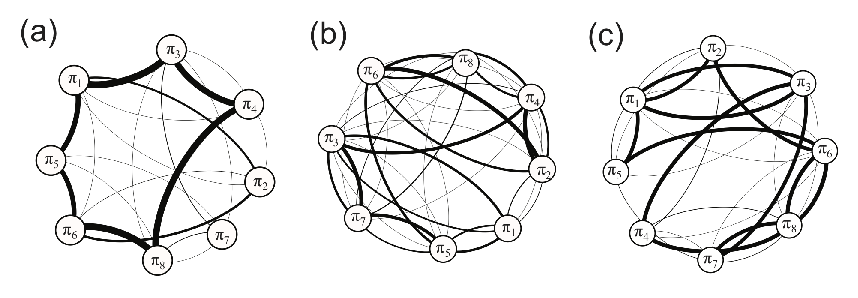
\includegraphics[width=\columnwidth]{Chapter05_TransitionNt/copt_jopt.eps}
	\caption{\small{Cross and joint ordinal pattern transition networks, which are reconstructed from two coupled R\"ossler systems in the non-sync regime \cite{Guo2018}. (a) Cross ordinal pattern transition network (COPT), (b) an alternative version of COPT, and (c) joint ordinal pattern transition network (JOPT). The directions of links have been suppressed for better visualizations. Reproduced from \cite{Guo2018}. } \label{fig:rosCOPT}}
\end{figure}	

		In an analogy, a joint ordinal pattern transition networks (JOPT) compares the relative speeds between two systems by the signs of $\Delta x_1(t) \cdot \Delta x_2(t), \Delta y_1(t) \cdot \Delta y_2(t)$ and $\Delta z_1(t) \cdot \Delta z_2(t)$ and the pattern definitions of a JOPT are summarized in Tab. \ref{tab:3DJOPT}. An example of JOPT is shown in Fig. \ref{fig:rosCOPT}(c).
\begin{table}[htb]
\centering
\begin{tabular}{|c|c|c|c|c|c|c|c|c|}
\hline
$\Pi$      & $\pi_1$ & $\pi_2$ & $\pi_3$ & $\pi_4$ & $\pi_5$ & $\pi_6$ & $\pi_7$
& $\pi_8$\\
\hline
$\Delta x_1 \cdot \Delta x_2$ & $+ $ & $+ $ & $+$ & $+$ & $ - $ & $ - $ & $-$ & $ - $\\
\hline
$\Delta y_1 \cdot \Delta y_2$ & $ + $ & $ + $ & $ -$ & $ -$ & $ + $ & $ + $ & $ -$ & $ -$\\
\hline
$\Delta z_1 \cdot \Delta z_2$ & $ + $ & $ - $ & $ +$ & $ -$ & $ + $ & $ - $ & $+$ & $ -$\\
\hline
\end{tabular}
\caption{Pattern definitions of a JOPT. Note that $``+"$ means a positive value while $``-"$ is for a negative value.  \label{tab:3DJOPT}}
\end{table}
In contrast to cross ordinal patterns, we notice that the joint ordinal patterns represent whether the respective variables of two systems show the same trend of changes or not, regardless of the magnitudes of the respective variables.

		The ideas of both COPT and JOPT have been particularly applied to analyze synchronization transitions \cite{Guo2018}. Note that a COPT and JOPT are two slightly different ways to construct networks from multivariate time series, providing complementary information. The ordinal patterns of a COPT are defined by considering the signs of the difference of $\Delta \vec{x}_1 - \Delta \vec{x}_2$ between two subsystems. In contrast, the ordinal patterns of a JOPT  are defined by the signs of the product of $\Delta \vec{x}_1 \cdot \Delta \vec{x}_2$. It is certain that the amplitudes of oscillations of different variables influence directly the definition of a COPT. However amplitudes become not important for a JOPT because only the signs of the product are considered. In addition, it is straightforward to generalize the ideas of JOPTs from two to three (or even $n$) coupled subsystems with an extended number of pattern definitions. However, it remains to be a big challenge for constructing a COPT for three coupled subsystems. 

		\subsubsection{Other approaches}
		For one dimensional symbol sequence, one may construct a directed symbol transition network \cite{Emmert2012}. Working with experimental data of $RR$-intervals from cardiac regulations, Makowiec {\textit{ et. al}} proposed to construct transitions networks from the subsequent increment series $\Delta RR_n = RR_n - RR_{n-1}$ \cite{Makowiec2013,Makowiec2013b,Makowiec2014b,Makowiec2015,Makowiec2015b,Makowiec2016}. In this series of work, they have demonstrated that transition network approaches are a powerful tool in quantifying the unique properties of the $RR$-interval time series of patients after heart transplant surgery. 
		
		When constructing ordinal partition transition networks by a sliding window scheme \cite{Small2013}, the ordinal pattern of the windowed sequence corresponds to one node of the network. Since the amplitude information is neglected, this approach may be combined with a transition network, where the nodes of the network are the binned amplitudes of the time series \cite{Sun2014}. More specifically, each time step $n$ is associated with a symbol-pair containing the amplitude information $\alpha (n)$ and the ordinal pattern $\pi (n)$. The former is calculated by binning the time series in the interval $[\min(\{ y_n\}), \max(\{ y_n \})]$ into $Q$ equal regions.  $\alpha(n)$ is then simply the bin number of $y_n$. Respectively, $\pi(n)$ is the ordinal pattern of the embedded vector $[y_n, y_{n+\tau}, \dots, y_{n+(L-1)\tau}]$. The symbol-pair at step $n$, $(\alpha(n), \pi(n))$, is then one node of the network and it is the connected by a directed link to the symbol-pair $(\alpha(n+1), \pi(n+1))$ of the successive time step. Furthermore, this algorithm has been combined with recurrence networks and surrogate networks, which has shown power in detecting weak nonlinearities in time series \cite{Laut2016}. 
		
		Coarse graining a financial time series, one may focus on the particular up-down behaviour of the volatility stock index series as presented in \cite{Li2006b,Li2007a}. More specifically, they symbolize time series by the parameter $\theta = \arctan \Delta x / \Delta t$, which characterizes the local increasing/decreasing velocity of the measurement. Then, the local velocities are coarse grained into four states ($R, r, d, D$), which correspond to violent-up meta, common-up meta, common down meta, and violent down meta patterns respectively. They found that the topological important nodes of the resulting transition networks play important roles in both information control and transport of stock market \cite{Li2007a}. 
		
		In a series of works by Gao \textit{et al.}\cite{Gao2014a,Gao2014,Gao2015}, they proposed a linear regression patterns transmission algorithm which captures the evolution of linear regression of bivariate time series. This algorithm has been demonstrated to be a useful tool to show the correlation mode transmission in crude oil spot price and future price \cite{Huang2015}. Based on reduced autoregressive models generated from time series, a proper directed transition network reconstruction algorithm has been proposed in \cite{Nakamura2012a}, such that the delay information has been successively captured by the transition behavior of the resulting network. Furthermore, proper surrogate method is required when extending these ideas from a univariate to multivariate time series analysis \cite{Nakamura2016}. 
		
		
	\subsection{Network interpretation of Markov chains}
